\documentclass[table,aspectratio=169]{beamer}
%% Choose aspect ratio:
% [aspectratio=43]  % 4:3 (default)
% [aspectratio=169] % 16:9, wide

\usetheme[minimal, nofont, noheadline]{tugraz2018}
%\usetheme[iaik,]{tugraz2018}
%% Choose main theme variant:
% [standard]        % standard (default)
% [iaik]       % with institute's graphical acronym on the left
% [minimal]         % with reduced visuals

%% Choose your font style:
%                   % Helvetica (default for Corporate Design)
% [webfont]         % Source Sans Pro (as used on tugraz.at)
% [nofont]          % no font loaded - Computer Modern Sans

%% Choose your department's color instead of TU Graz tugred (optional):
% [arch]            % 
% [bau]             %
% [etit]            %
% [mbww]            %
% [tcvp]            %
% [mpug]            %
% [infbio]          %


\usepackage[utf8]{inputenc}
\usepackage[english]{babel}
%% Choose your language:
% [ngerman]   % German
% [english]   % English


%% Add your own packages, macros, etc.
\usepackage{xcolor,colortbl, soul}
\usepackage{booktabs,nicematrix}
\usepackage{rotating}
\usepackage[style=alphabetic,backend=biber]{biblatex} % Bibliography
\addbibresource{\jobname.bib}                         % Bibliography
\usepackage{fontawesome}
\usepackage{filecontents}
\usepackage{setspace}
\usepackage{subcaption}
\usepackage{multirow}
\usepackage{bm}
\usepackage{pgfplots}
\usepackage[linesnumbered,ruled,vlined]{algorithm2e}
\usepackage{framed, color}
\usepackage{mathtools}
\usepackage{graphicx}
\usepackage{circledsteps}
\usepackage{clefia,warp}


\tikzset{
    invisible/.style={opacity=0.2},
    visible on/.style={alt={#1{}{invisible}}},
    alt/.code args={<#1>#2#3}{%
        \alt<#1>{\pgfkeysalso{#2}}{\pgfkeysalso{#3}}%
    }
}

\usetikzlibrary{positioning}
\usetikzlibrary{calc,patterns, arrows.meta, shapes.geometric, positioning, decorations.markings}
\usetikzlibrary{cipher}
\usetikzlibrary{external}
\tikzexternalize[prefix=tikz-ext/, only named=true, aux in dpth=true]
\setbeamersize
{
	text margin left=0.4cm,
	text margin right=0.4cm
}

%% Enter presentation metadata
\title{Throwing Boomerangs into Feistel Structures
\\
\small{Application to \cipher{CLEFIA}, \cipher{WARP}, \cipher{LBlock}, \cipher{LBlock-s} and \cipher{TWINE}}}
\author{\underline{\textbf{Hosein Hadipour}} \and Marcel Nageler \and Maria Eichlseder}
\date{FSE 2023 - Kobe, Japan}
%\institute{IAIK}
\instituteurl{hossein.hadipour@iaik.tugraz.at}

%% Macros
\newcommand{\sparen}{\vspace*{-.3cm}}
% \newcommand{\cipher}[1]{\textsc{#1}}

%% Colors
\definecolor{diffred}{HTML}{f70146}
\definecolor{diffpurple}{HTML}{6c2f91}
\definecolor{diffmid}{HTML}{5191c1}
\definecolor{diffgray}{HTML}{a5a5a5}
\definecolor{diffblue}{HTML}{285f82}
\definecolor{diffgreen}{HTML}{78b473}
\definecolor{diffyellow}{HTML}{e59352}
\definecolor{diffcyan}{HTML}{77babf}
\definecolor{diffhead}{HTML}{245b78}
\definecolor{diffbody}{HTML}{e2e9ed}

\colorlet{ps}{diffmid!70}
\colorlet{gs}{diffgreen!50}

\begin{document}

\begin{frame}[plain]
  \maketitle
\end{frame}


\section*{Research Gap and Our Contributions}
\sectionheader[\huge\color{tug}\faBook]{Research Gap and Our Contributions}
\begin{frame}{Motivation and Our Contributions}
\onslide<1->{
Research gap:
}
\begin{itemize}
	\footnotesize
	\item<1->[\faExpeditedssl] The lack of a tool to automatically find boomerang distinguishers for Feistel cipher
\end{itemize}
\onslide<2->{
Contributions:
}
\begin{itemize}
	\footnotesize
	\item<2->[\faFighterJet] Providing an easy to use and fast method to find boomerang distinguishers
	\item<3->[\faCheckCircleO] We applied our method to \cipher{CLEFIA}, \cipher{WARP}, \cipher{LBlock}, and \cipher{TWINE}
\begin{itemize}
	\footnotesize
	\item<4->[\faLineChart] We improved the boomerang distinguisher of \cipher{WARP} by 2 rounds
	\item<5->[\faLineChart] We improved the boomerang distinguisher/attack  of \cipher{CLEFIA} by 1 round
\end{itemize}
	\item<6->[\faWrench] Our method is applicable to any strongly aligned (Sbox-based) block cipher, e.g., SKINNY
\end{itemize}
\end{frame}


\section*{}
\begin{frame}{Outline}
  \tableofcontents
\end{frame}


\section{Effective Parameters in the Success Probability of Boomerang Distinguishers}
\sectionheader[\huge\color{tug}\faBook]{Effective Parameters in the Success Probability of \\Boomerang Distinguishers}

\begin{frame}{Boomerang Distinguishers \cite{fse_Wagner99}}
\vspace{-0.55cm}
\begin{columns}
\column[c]{0.4\textwidth}
\centering
\resizebox{1.3\textwidth}{!}{
\begin{tikzpicture}[baseline=1cm, very thick]
\pgfmathsetmacro{\hstep}{0.9};
\pgfmathsetmacro{\vstep}{1.8};
\pgfmathsetmacro{\length}{8*\hstep};
\pgfmathsetmacro{\halflength}{\length/2};
\pgfmathsetmacro{\hight}{1};
\pgfmathsetmacro{\halfhight}{\hight/2};
\node[] (r1) at (0, 0) {$\Delta$};
\node[right=\hstep of r1] (c1) {};
\node[right=\halflength of c1] (c2) {};
\node[right=\halflength of c2] (c3) {};
\node[right=\hstep of c3] (c4) {$\nabla$};
\visible<1->{%
\draw[rounded corners=3pt] ($(c1) + (0, -\halfhight)$) rectangle ($(c3) + (0, \halfhight)$) node[pos=.5] {$E:\mathbb{F}_{2}^{n} \rightarrow \mathbb{F}_{2}^{n}$};
\draw[->] (r1) -- (c1);
\draw[->] (c3) -- (c4);
\visible<1>{%
\node[below=2*\halfhight of c2] (text) {$0 \lneq \Pr\{\Delta \xrightarrow{E} \nabla\} \lll 2^{-n}$};
}}
\visible<2->{%
\draw[rounded corners=3pt, fill=white] ($(c1) + (0, -\halfhight)$) rectangle ($(c3) + (0, \halfhight)$);
\draw[gray] ($(c2) + (0, -\halfhight)$) -- ($(c2) + (0, \halfhight)$);
\node[] at ($0.5*(c1) + 0.5*(c2)$) {$E_{0}$};
\node[] at ($0.5*(c2) + 0.5*(c3)$) {$E_{1}$};
% Shift the axes down by \vstep units
\node[below=\vstep of r1] (r1) {$\Delta_{1}$};
\node[right=\hstep of r1] (c1) {};
\node[right=\halflength of c1] (c2) {};
\node[right=\halflength of c2] (c3) {};
\draw[rounded corners=3pt, fill=tugred] ($(c1) + (0, -\halfhight)$) rectangle ($(c2) + (0, \halfhight)$) node[pos=.5] {$E_{0}$};
\node[right=\hstep of c2] (temp) {$\Delta_{2}$};
\draw[->] (r1) -- (c1);
\draw[->] (c2) -- (temp);
\node[] at ($0.5*(c1) + 0.5*(c2) + (0, \hstep)$) {$p = \Pr\{\Delta_{1} \xrightarrow{E_{0}} \Delta_{2}\}$};
% Shift the axes down by \vstep units
\node[below=\vstep of r1] (r1) {};
\node[right=\hstep of r1] (c1) {};
\node[right=\halflength of c1] (c2) {};
\node[right=\halflength of c2] (c3) {};
\draw[rounded corners=3pt, fill=tugblue] ($(c2) + (0, -\halfhight)$) rectangle ($(c3) + (0, \halfhight)$) node[pos=.5] {$\textcolor{white}{E_{1}}$};
\node[left=\hstep of c2] (temp1) {$\nabla_{2}$};
\node[right=\hstep of c3] (temp2) {$\nabla_{3}$};
\draw[->] (temp1) -- (c2);
\draw[->] (c3) -- (temp2);
\node[] at ($0.5*(c2) + 0.5*(c3) + (0, \hstep)$) {$q = \Pr\{\nabla_{2} \xrightarrow{E_{1}} \nabla_{3}\}$};
% Shift the axes down by \halfhight+0.2 units
\node[below=\halfhight+0.2 of r1] (r1) {};
\node[right=\hstep of r1] (c1) {};
\node[right=\halflength of c1] (c2) {};
\visible<6>{
\node[fill=tugyellow, below=0.5 of c2] (pnode) {{\large$\textcolor{black}{\Pr\{p_{3} \oplus p_{4} = \Delta_{1}\} = p^{2} q^{2}}$}};
}
% \node[fill=tugyellow] at (c2) {$p^{2}q^{2} \ggg 2^{-n}$};
}
\end{tikzpicture}}
\column[c]{0.6\textwidth}
\begin{flushright}
\resizebox*{0.7\textwidth}{!}{
\begin{tikzpicture}[yscale=1,xscale=1, baseline=-1cm, thick]
\pgfmathsetmacro{\deltai}{3.3};
\pgfmathsetmacro{\nablao}{3.5};
\pgfmathsetmacro{\depth}{6};
\pgfmathsetmacro{\halfdepth}{\depth/2};
\pgfmathsetmacro{\quarterfdepth}{\depth/4};
\pgfmathsetmacro{\verticaldownshift}{1};
\visible<3->{%
\node (p1) at (0, 0) {$p_{1}$};
\node (p2) at ($(p1) + (\deltai, -\verticaldownshift)$) {$p_{2}$};
\node[below=\halfdepth of p1] (x1) {$x_{1}$};
\node[below=\halfdepth of p2] (x2) {$x_{2}$};
\node[box, below=\quarterfdepth of p1.center, fill=tugred] (e0l1) {$E_{0}$};
\node[box, below=\quarterfdepth of p2.center, fill=tugred] (e0l2) {$E_{0}$};
\node[below=\halfdepth of x1] (c1) {$c_{1}$};
\node[below=\halfdepth of x2] (c2) {$c_{2}$};
\node[box, below=\quarterfdepth of x1.center, fill=tugblue] (e1l1) {$\textcolor{white}{E_{1}}$};
\node[box, below=\quarterfdepth of x2.center, fill=tugblue] (e1l2) {$\textcolor{white}{E_{1}}$};
\draw[<->, dashed, tugred] (p1) -- node[above] {$\Delta_{1}$} (p2);
\draw[<->, dashed, tugred] (x1) -- node[below] {$\Delta_{2}$} (x2);
\draw[->] (p1) -- (e0l1) -- (x1);
\draw[->] (x1) -- (e1l1) -- (c1);
\draw[->] (p2) -- (e0l2) -- (x2);
\draw[->] (x2) -- (e1l2) -- (c2);
\node[right=\nablao of c1] (c3) {\textcolor{white}{$c_{3}$}};
\node[right=\nablao of c2] (c4) {\textcolor{white}{$c_{4}$}};
}

\visible<4->{%
\node[right=\nablao of c1] (c3) {$c_{3}$};
\node[right=\nablao of c2] (c4) {$c_{4}$};
\draw[<->, dashed, tugblue] (c1) -- node[above] {$\nabla_{3}$} (c3);
\draw[<->, dashed, tugblue] (c2) -- node[above] {$\nabla_{3}$} (c4);
}

\visible<5->{%
\node[right=\nablao of x1] (x3) {$x_{3}$};
\node[right=\nablao of x2] (x4) {$x_{4}$};
\node[box, below=\quarterfdepth of x3.center, fill=tugblue] (e1r1) {$\textcolor{white}{E_{1}}$};
\node[box, below=\quarterfdepth of x4.center, fill=tugblue] (e1r2) {$\textcolor{white}{E_{1}}$};
\draw[<->, dashed, tugblue] (x1) -- node[above] {$\nabla_{2}$} (x3);
\draw[<->, dashed, tugblue] (x2) -- node[below] {$\nabla_{2}$} (x4);
\draw[->] (c3) -- (e1r1) -- (x3);
\draw[->] (c4) -- (e1r2) -- (x4);
}
\visible<6>{
\node[right=\nablao of p1] (p3) {$p_{3}$};
\node[right=\nablao of p2] (p4) {$p_{4}$};
\node[box, below=\quarterfdepth of p3.center, fill=tugred] (e0r1) {$E_{0}$};
\node[box, below=\quarterfdepth of p4.center, fill=tugred] (e0r2) {$E_{0}$};
\draw[->] (x3) -- (e0r1) -- (p3);
\draw[->] (x4) -- (e0r2) -- (p4);

\draw[<->, dashed, tugred] (x3) -- node[above] {$\Delta_{2}$} (x4);
\draw[<->, dashed, tugred] (p3) -- node[above] {$\Delta_{1}$} (p4);
}
\end{tikzpicture}}
\end{flushright}
\end{columns}
\end{frame}

% \begin{frame}{Dependencies and Boomerang Switch}
% \begin{columns}
% \column[c]{0.5\textwidth}
% \centering
% \scalebox{0.6}{
%   \begin{tabular}{|c|c|c|c|c|c|c|c|c|c|c|c|c|c|c|c|c|}
%     \hline
%     $x$   & $\mathtt 0$ & $\mathtt 1$ & $\mathtt 2$ & $\mathtt 3$ & $ \mathtt 4$ & $\mathtt 5$ & $\mathtt 6$ & $\mathtt 7$ & $ \mathtt 8$ & $\mathtt 9$ & $\mathtt a$ & $\mathtt b$ & $\mathtt c$ & $\mathtt d$ & $\mathtt e$ & $\mathtt f$ \\
%     \hline
%     $\mathcal S(x)$ & $\mathtt c$ & $\mathtt a$ & $\mathtt  d$ & $\mathtt 3$ & $\mathtt e$ & $\mathtt b$ & $\mathtt f$ & $\mathtt 7$ & $\mathtt 8$ & $\mathtt 9$ & $\mathtt 1$ & $\mathtt 5$ & $\mathtt 0$ & $\mathtt 2$ & $\mathtt 4$ & $\mathtt 6$\\
%     \hline
%   \end{tabular}
% }
% \onslide<2-3>{%
% \[Pr(\textcolor{tugred}{\Delta} = \texttt{3} \rightarrow \textcolor{tugred}{\Delta'} = \texttt{6}) = 2^{-2}\]
% }
% \onslide<3-3>{%
% \[Pr(\textcolor{tugred}{\Delta} = \texttt{3} \rightleftarrows \textcolor{tugblue}{\nabla} = \texttt{6}) = 0\]
% }
% \visible<4-5>{
% \[Pr(\textcolor{tugred}{\Delta} = \texttt{2} \rightarrow \textcolor{tugred}{\Delta'} = \texttt{2}) = 0\]
% }
% \visible<5-5>{%
% \[Pr(\textcolor{tugred}{\Delta} = \texttt{2} \rightleftarrows \textcolor{tugblue}{\nabla} = \texttt{2}) = 1\]	
% }
% \column[c]{0.5\textwidth}
% \centering
% \begin{figure}
% \centering
% \begin{tikzpicture}[yscale=1,xscale=1, baseline=-1cm, thick]
% \pgfmathsetmacro{\deltai}{2.8};
% \pgfmathsetmacro{\nablao}{3.2};
% \pgfmathsetmacro{\depth}{5};
% \pgfmathsetmacro{\halfdepth}{\depth/2};
% \pgfmathsetmacro{\quarterfdepth}{\depth/4};
% \pgfmathsetmacro{\verticaldownshift}{2};
% \visible<2->{%}
% \node (x1) at (0, 0) {$x_{1}$};
% \node (x2) at ($(x1) + (\deltai, -\verticaldownshift)$) {$x_{2}$};
% \node[below=\halfdepth of x1] (y1) {$y_{1}$};
% \node[below=\halfdepth of x2] (y2) {$y_{2}$};
% \node[box, below=\quarterfdepth of x1.center, fill=tuggreen] (e1l1) {$S$};
% \node[box, below=\quarterfdepth of x2.center, fill=tuggreen] (e1l2) {$S$};
% \draw[->] (x1) -- (e1l1) -- (y1);
% \draw[->] (x2) -- (e1l2) -- (y2);
% \node[right=\nablao of y1] (y3) {$y_{3}$};
% \node[right=\nablao of y2] (y4) {$y_{4}$};
% \node[right=\nablao of x1] (x3) {$x_{3}$};
% \node[right=\nablao of x2] (x4) {$x_{4}$};
% \node[box, below=\quarterfdepth of x3.center, fill=tuggreen] (e1r1) {$S$};
% \node[box, below=\quarterfdepth of x4.center, fill=tuggreen] (e1r2) {$S$};
% \draw[->] (y3) -- (e1r1) -- (x3);
% \draw[->] (y4) -- (e1r2) -- (x4);
% \draw[<->, dashed, tugred] (x1) -- node[above] {$\Delta$} (x2);
% \draw[<->, dashed, tugred] (x3) -- node[above] {$\Delta$} (x4);
% }
% \visible<2-3>{%
% \draw[<->, dashed, tugred] (y1) -- node[above] {$\Delta'$} (y2);
% \draw[<->, dashed, tugred] (y3) -- node[above] {$\Delta'$} (y4);
% }
% \visible<3>{%
% \draw[<->, dashed, tugblue] (y1) -- node[above] {$\nabla$} (y3);
% \draw[<->, dashed, tugblue] (y2) -- node[above] {$\nabla$} (y4);
% }
% % \visible<4>{%
% % \draw[<->, dashed, tugblue] (y1) -- node[above] {$\nabla$} (y3);
% % \draw[<->, dashed, tugblue] (y2) -- node[above] {$\nabla$} (y4);
% % \draw[<->, tugred, dashed] (x3) -- node[above] {$\textcolor{tugred}{\Delta}$} (x4);
% % }
% \visible<4->{%
% \draw[<->, dashed, tugred] (y1) -- node[above] {$\Delta'$} (y2);
% \draw[<->, dashed, tugred] (y3) -- node[above] {$\Delta'$} (y4);
% }
% \visible<5>{%
% \draw[<->, dashed, tugblue] (y1) -- node[above] {$\nabla$} (y3);
% \draw[<->, dashed, tugblue] (y2) -- node[above] {$\nabla$} (y4);
% \draw[<->, tugred, dashed] (x3) -- node[above] {$\textcolor{tugred}{\Delta}$} (x4);
% }
% \end{tikzpicture}
% \end{figure}
% \end{columns}
% \end{frame}


\begin{frame}{Sandwiching the Differentials! \cite{conf_crypto_DunkelmanKS10}}
% \vspace{-0.4cm}
\begin{columns}
\column[c]{0.5\textwidth}
\centering
\only<1->{%
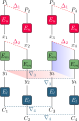
\includegraphics[width=0.55\textwidth]{./figures/sandwich.pdf}
}
\column[c]{0.5\textwidth}
\centering
\only<1>{%

\includegraphics[width=0.65\textwidth]{./figures/realsandwich.pdf}
}
% \only<3>{%
% 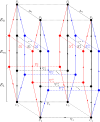
\includegraphics[width=0.64\textwidth]{./figures/sandwichcluster.pdf}
% }
\only<2>{%
\begin{gather*}
\Pr(P_{3} \oplus P_{4} = \textcolor{tugred}{\Delta_{1}}) \approx p^{2}\times r \times q^{2}\\
r = \Pr(\textcolor{tugred}{\Delta_{2}} \rightleftarrows \textcolor{tugblue}{\nabla_{3}})
\end{gather*}
}
\end{columns}
% \only<3>{%
% {\small
% \[\Pr\left(P_{3} \oplus P_{4} = \Delta_{1}\right) = \sum_{\Delta_{2}, \Delta_{2}', \nabla_{3}, \nabla_{3}'} p_{\nabla{3}}\times p_{\nabla_{3}'} \times r(\Delta_{2}, \Delta_{2}', \nabla_{3}, \nabla_{3}') \times q_{\nabla_{3}} \times q_{\nabla_{3}'}\]
% }
% }
\end{frame}

\begin{frame}{Boomerang Switch For SPN Block Ciphers}
\vspace{-0.5cm}
\begin{figure}
\centering
\begin{tikzpicture}[yscale=0.6,xscale=1, baseline=-1cm, thin]
\pgfmathsetmacro{\deltai}{2.6};
\pgfmathsetmacro{\nablao}{2.8};
\pgfmathsetmacro{\depth}{5};
\pgfmathsetmacro{\halfdepth}{\depth/2};
\pgfmathsetmacro{\quarterfdepth}{\depth/4};
\pgfmathsetmacro{\verticaldownshift}{1.2};
\node (x1) at (0, 0) {$x_{1}$};
\node (x2) at ($(x1) + (\deltai, -\verticaldownshift)$) {$x_{2}$};
\node[below=\halfdepth of x1] (y1) {$y_{1}$};
\node[below=\halfdepth of x2] (y2) {$y_{2}$};
\node[box, below=\quarterfdepth of x1.center, fill=tuggreen] (e1l1) {$S$};
\node[box, below=\quarterfdepth of x2.center, fill=tuggreen] (e1l2) {$S$};
\draw[<->, dashed, red] (x1) -- node[above] {$\Delta$} (x2);
\draw[->] (x1) -- (e1l1) -- (y1);
\draw[->] (x2) -- (e1l2) -- (y2);
\node[right=\nablao of y1] (y3) {$y_{3}$};
\node[right=\nablao of y2] (y4) {$y_{4}$};
\draw[<->, dashed, blue] (y1) -- node[above] {$\nabla$} (y3);
\draw[<->, dashed, blue] (y2) -- node[above] {$\nabla$} (y4);
\node[right=\nablao of x1] (x3) {$x_{3}$};
\node[right=\nablao of x2] (x4) {$x_{4}$};
\node[box, below=\quarterfdepth of x3.center, fill=tuggreen] (e1r1) {$S^{-1}$};
\node[box, below=\quarterfdepth of x4.center, fill=tuggreen] (e1r2) {$S^{-1}$};
\draw[->] (y3) -- (e1r1) -- (x3);
\draw[->] (y4) -- (e1r2) -- (x4);
\draw[<->, red, dashed] (x3) -- node[above] {$\textcolor{red}{\Delta}$} (x4);
\end{tikzpicture}
\end{figure}
% \only<1>{
% {\small 
% \[r = r(\textcolor{red}{\Delta}, \textcolor{blue}{\nabla}) = \Pr\{S^{-1}(S(x) \oplus \textcolor{blue}{\nabla}) \oplus S^{-1}(S(x \oplus \textcolor{red}{\Delta}) \oplus \textcolor{blue}{\nabla}) = \textcolor{red}{\Delta}\}\]
% }
% }
\only<1->{
{\small
\[\texttt{BCT}(\textcolor{red}{\Delta}, \textcolor{blue}{\nabla}) \coloneqq \#\{x\in \mathbb{F}_{2}^{n}\,|\,S^{-1}\left(S(x) \oplus \textcolor{blue}{\nabla}\right) \oplus S^{-1}(S(x \oplus \textcolor{red}{\Delta}) \oplus \textcolor{blue}{\nabla}) = \textcolor{red}{\Delta}\}\]
}
}
\onslide<2->{
{\small
\[\texttt{BCT}(\textcolor{red}{0}, \textcolor{blue}{\nabla}) = \texttt{BCT}(\textcolor{red}{\Delta}, \textcolor{blue}{0}) = 2^{n}\]
}
}
\end{frame}

\begin{frame}{Boomerang Switch For Feistel Ciphers}
\centering
\resizebox*{0.65\textwidth}{!}{
\begin{tikzpicture}[xscale=1,yscale=1, thick,>=latex]
	\pgfmathsetmacro{\deltai}{2.7};
	\pgfmathsetmacro{\nablao}{5.1};
	\pgfmathsetmacro{\depth}{4};
	\pgfmathsetmacro{\quarterdepth}{\depth/4};
	\pgfmathsetmacro{\oneeithdepth}{\depth/8};
	\pgfmathsetmacro{\halfdepth}{\depth/2};
	\pgfmathsetmacro{\verticaldownshift}{.75};
	\pgfmathsetmacro{\horizshift}{1.5};
	\pgfmathsetmacro{\quarterhorizshift}{\horizshift/4};
	\node (X1) at (0, 0) {$x_{1}$};
	\node (X2) at ($(X1) + (\deltai, -\verticaldownshift)$) {$x_{2}$};
	\node[right=\nablao of X1] (X3) {$x_{3}$};
	\node[right=\nablao of X2] (X4) {$x_{4}$};
	\coordinate[below=\halfdepth of X1] (U1);
	\coordinate[below=\halfdepth of X2] (U2);
	\coordinate[below=\halfdepth of X3] (U3);
	\coordinate[below=\halfdepth of X4] (U4);
	\node[tee, above=\quarterdepth of U1] (M1) {};
	\node[tee, above=\quarterdepth of U2] (M2) {};
	\node[tee, above=\quarterdepth of U3] (M3) {};
	\node[tee, above=\quarterdepth of U4] (M4) {};
	\node[box, right=\quarterhorizshift of M1, fill=tuggreen] (S1) {$S$};
	\node[box, right=\quarterhorizshift of M2, fill=tuggreen] (S2) {$S$};
	\node[box, right=\quarterhorizshift of M3, fill=tuggreen] (S3) {$S$};
	\node[box, right=\quarterhorizshift of M4, fill=tuggreen] (S4) {$S$};
	\node[xor, right=\horizshift of M1, gray] (XOR1) {};
	\node[xor, right=\horizshift of M2, gray] (XOR2) {};
	\node[xor, right=\horizshift of M3, gray] (XOR3) {};
	\node[xor, right=\horizshift of M4, gray] (XOR4) {};
	\coordinate[above=\quarterdepth of XOR1] (Xp1);
	\coordinate[above=\quarterdepth of XOR2] (Xp2);
	\coordinate[above=\quarterdepth of XOR3] (Xp3);
	\coordinate[above=\quarterdepth of XOR4] (Xp4);
	\coordinate[below=\quarterdepth of XOR1] (Up1);
	\coordinate[below=\quarterdepth of XOR2] (Up2);
	\coordinate[below=\quarterdepth of XOR3] (Up3);
	\coordinate[below=\quarterdepth of XOR4] (Up4);
	\coordinate[below=\oneeithdepth of U1] (Vp1);
	\coordinate[below=\oneeithdepth of U2] (Vp2);
	\coordinate[below=\oneeithdepth of U3] (Vp3);
	\coordinate[below=\oneeithdepth of U4] (Vp4);
	\coordinate[below=\quarterdepth of U1] (Yp1);
	\coordinate[below=\quarterdepth of U2] (Yp2);
	\coordinate[below=\quarterdepth of U3] (Yp3);
	\coordinate[below=\quarterdepth of U4] (Yp4);
	%\node[below right=\quarterdepth and \horizshift of U1] (Y1) {$x_{1}$};
	%\node[below right=\quarterdepth and \horizshift of U2] (Y2) {$x_{2}$};
	%\node[below right=\quarterdepth and \horizshift of U3] (Y3) {$x_{3}$};
	%\node[below right=\quarterdepth and \horizshift of U4] (Y4) {$x_{4}$};
	%\coordinate[above=\oneeithdepth of Y1] (V1);
	%\coordinate[above=\oneeithdepth of Y2] (V2);
	%\coordinate[above=\oneeithdepth of Y3] (V3);
	%\coordinate[above=\oneeithdepth of Y4] (V4);
	\coordinate (V1) at (Up1|-Vp1);
	\coordinate (V2) at (Up2|-Vp2);
	\coordinate (V3) at (Up3|-Vp3);
	\coordinate (V4) at (Up4|-Vp4);
	\node[below] (Y1) at (V1|-Yp1) {$x_{1}$};
	\node[below] (Y2) at (V2|-Yp2) {$x_{2}$};
	\node[below] (Y3) at (V3|-Yp3) {$x_{3}$};
	\node[below] (Y4) at (V4|-Yp4) {$x_{4}$};
	\draw[next, rounded corners=2pt] (X1) -- (U1) -- (V1) -- (Y1);
	\draw[next, rounded corners=2pt] (X2) -- (U2) -- (V2) -- (Y2);
	\draw[next, rounded corners=2pt] (Y3) -- (V3) -- (U3) -- (X3);
	\draw[next, rounded corners=2pt] (Y4) -- (V4) -- (U4) -- (X4);
	\draw[<->, dashed, tugred] (X1) -- node[above]{$\Delta$} (X2);
	\draw[<->, dashed, tugred] (X3) -- node[above]{$\Delta$} (X4);
	\draw[<->, dashed, tugblue] (Y1) -- node[above]{$\nabla$} (Y3);
	\draw[<->, dashed, tugblue] (Y2) -- node[above]{$\nabla$} (Y4);
	\draw[->] (M1) -- (S1) -- (XOR1);
	\draw[->] (M2) -- (S2) -- (XOR2);
	\draw[->] (M3) -- (S3) -- (XOR3);
	\draw[->] (M4) -- (S4) -- (XOR4);
	\draw[next, dashed, gray, rounded corners=2pt] (Xp1) -- (XOR1) -- (Up1) -- (Vp1) -- (Yp1);
	\draw[next, dashed, gray, rounded corners=2pt] (Xp2) -- (XOR2) -- (Up2) -- (Vp2) -- (Yp2);
	\draw[next, dashed, gray, rounded corners=2pt] (Yp3) -- (Vp3) -- (Up3) -- (XOR3) -- (Xp3);
	\draw[next, dashed, gray, rounded corners=2pt] (Yp4) -- (Vp4) -- (Up4) -- (XOR4) -- (Xp4);
\end{tikzpicture}
}
\[\texttt{FBCT}(\textcolor{tugred}{\Delta}, \textcolor{tugblue}{\nabla}) \coloneqq \#\{x\in \mathbb{F}_{2}^{n}: S(x) \oplus S(x \oplus \textcolor{tugred}{\Delta}) \oplus S(x\oplus \textcolor{tugblue}{\nabla}) \oplus S(x \oplus \textcolor{tugred}{\Delta} \oplus \textcolor{tugblue}{\nabla}) = 0\}\]
\pause
\[\texttt{FBCT}(\textcolor{tugred}{\Delta}, \textcolor{tugblue}{0}) = \texttt{FBCT}(\textcolor{tugred}{0}, \textcolor{tugblue}{\nabla}) = 2^{n}\]
\end{frame}

\begin{frame}{Building Deterministic Boomerang from Impossible Trails \cite{tosc_HadipourBS21}}
\begin{minipage}[l]{0.8\linewidth}
\begin{overprint}
\only<1>{
\includegraphics[width=0.9\textwidth]{./figures/skinny_tk2_11r.pdf}
}
\only<2>{
\includegraphics[width=0.9\textwidth]{./figures/upper_trail.pdf}
}
\only<3>{
\includegraphics[width=0.9\textwidth]{./figures/lower_trail.pdf}
}
\only<4>{
\includegraphics[width=0.9\textwidth]{./figures/bmd.pdf}
}
\end{overprint}
\end{minipage}\hspace{-0.8cm} 
\begin{minipage}[l]{0.2\linewidth}
\begin{itemize}
\item<2-> $\textcolor{tugred}{p = 2^{-146}}$ {\scriptsize (impossible due to dependencies \cite{journals_tosc_PeyrinT22})}
\item<3-> $\textcolor{tugblue}{q = 2^{-179}}$ {\scriptsize (impossible due to dependencies \cite{journals_tosc_PeyrinT22})}
\item<4-> $\Pr_{\texttt{boom}} = 1$
\end{itemize}
\end{minipage}
\end{frame}

\begin{frame}{Effective Parameters in $p^{2}q^{2}r$ Formula}
\begin{figure}
\centering
\begin{tikzpicture}[xscale=1,yscale=1, thick,>=latex]
\pgfmathsetmacro{\EO}{4};
\pgfmathsetmacro{\HEO}{\EO/2};
\pgfmathsetmacro{\EM}{3};
\pgfmathsetmacro{\HEM}{\EM/2};
\pgfmathsetmacro{\gap}{1};
\pgfmathsetmacro{\W}{1};
\coordinate (u0) at (0, 0);
\coordinate[right=\gap of u0] (u1);
\coordinate[right=\EO of u1] (u2);
\coordinate[right=\gap of u2] (u3);
\coordinate[right=\EM of u3] (u4);
\coordinate[below=3*\gap of u3] (l0);
\coordinate[right=\EM of l0] (l1);
\coordinate[right=\gap of l1] (l2);
\coordinate[right=\EO of l2] (l3);
\coordinate[right=\gap of l3] (l4);

\only<1->{
\draw[rounded corners] ($(u1) + (0, -\W)$) rectangle ($(u2) + (0, \W)$) node[pos=.5] {$E_{0}$};
}
\visible<2->{
\draw[->] (u0) --node[above]{$\Delta_{1}$} (u1);
\draw[rounded corners, fill=tugred] ($(u1) + (0, -\W)$) rectangle ($(u2) + (0, \W)$) node[pos=.5] {$E_{0}$};
\draw[->] (u2) --node[above]{$\Delta_{2}$} (u3);
\node at ($(u1) + (\HEO, -1.5\W)$) {{\large \textcolor{tugred}{$p$}}};
}
\visible<1->{
\draw[rounded corners] ($(u3) + (0, -\W)$) rectangle ($(u4) + (0, \W)$) node[pos=.5] {$E_{m}$};
\draw[rounded corners] ($(l0) + (0, -\W)$) rectangle ($(l1) + (0, \W)$) node[pos=.5] {$E_{m}$};
}
\visible<4->{
\draw[rounded corners, fill=tuggreen] ($(u3) + (0, -\W)$) rectangle ($(u4) + (0, \W)$) node[pos=.5] {$E_{m}$};
\node at ($(u3) + (\HEM, -1.5\W)$) {{\large $r$}};
\draw[rounded corners, fill=tuggreen] ($(l0) + (0, -\W)$) rectangle ($(l1) + (0, \W)$) node[pos=.5] {$E_{m}$};
}
\visible<1->{
\draw[rounded corners] ($(l2) + (0, -\W)$) rectangle ($(l3) + (0, \W)$) node[pos=.5] {$E_{1}$};
}
\visible<3->{
\draw[<-] (l1) --node[below]{$\nabla_{3}$} (l2);
\draw[rounded corners, fill=tugblue] ($(l2) + (0, -\W)$) rectangle ($(l3) + (0, \W)$) node[pos=.5] {\textcolor{white}{$E_{1}$}};
\node at ($(l2) + (\HEO, +1.5\W)$) {{\large \textcolor{tugblue}{$q$}}};
\draw[<-] (l3) --node[below]{$\nabla_{4}$} (l4);
}

\end{tikzpicture}
\end{figure}
\visible<5>{
\begin{itemize}
\item[\faWarning] {\small Active S-boxes in $E_{0}, E_{1}$ are more expensive than common active S-boxes in $E_{m}$}
\end{itemize}
}
\end{frame}

\section{Our Method to Search for Boomerang Distinguishers}
\sectionheader[\huge\color{tug}\faCogs]{Our Method to Search for Boomerang Distinguishers}

\begin{frame}{Our Method to Find Boomerang Distinguishers}
	Our method has three steps:
	\begin{itemize}		
		\item<1->[\faArrowCircleRight] Find good truncated upper and lower trails:
		\begin{itemize}
			\item<2-> minimize number of active S-boxes in outer parts, i.e., $E_{0}$, and  $E_{1}$
			\item<2-> minimize number of common active S-boxes in the middle part, i.e., $E_{m}$
		\end{itemize}		
		\item<3->[\faArrowCircleRight] Instantiate discovered truncated trails with concrete differential trails
		\item<4->[\faArrowCircleRight] Compute $p$, $q$ and $r$ to derive the entire probability, i.e.,  $p^{2}q^{2}r$
	\end{itemize}
\end{frame}

\begin{frame}{Find Good Truncated Upper and Lower Trails}
\vspace{-0.5cm}
\begin{figure}
\centering
\begin{tikzpicture}[yscale=1,xscale=1,baseline=0, decoration={
	markings,
	mark=at position 0.5 with {\arrow{>>}}}]
\pgfmathsetmacro{\hstep}{4}
\pgfmathsetmacro{\vstep}{1.2}
\pgfmathsetmacro{\halfvstep}{\vstep/2}
\pgfmathsetmacro{\quartervstep}{\vstep/4}
\pgfmathsetmacro{\halfhstep}{\hstep/2}
\pgfmathsetmacro{\quarterhstep}{\hstep/4}

\visible<1->{
	\node[overlay] (c1) at (0, 0) {};
	\node[overlay, right=\hstep of c1] (c2) {};
	\node[overlay, right=\hstep of c2] (c3) {};
	\node[overlay, right=\hstep of c3] (c4) {};		
	\draw[rounded corners=2pt] ($(c1) + (0, -\halfvstep)$) rectangle ($(c4) + (0, \halfvstep)$) node[pos=0.5] {\only<1>{$E$}\only<2->{$E_{m}$}};
	\draw[<->, dashed, white] ($(c1) + (0, \halfvstep + 0.1)$) -- node[above] {$r_{0}$} ($(c2) + (0,
	\halfvstep + 0.1)$);
}
\visible<2-5>{
	\draw[rounded corners=2pt] ($(c1) + (0, -\halfvstep)$) rectangle ($(c4) + (0, \halfvstep)$);
	\draw[] ($(c2) + (0, -\halfvstep)$) -- ($(c2) + (0, \halfvstep + 0.2)$);
	\draw[] ($(c3) + (0, -\halfvstep)$) -- ($(c3) + (0, \halfvstep + 0.2)$);
	\draw[<->, dashed] ($(c1) + (0, \halfvstep + 0.1)$) -- node[above] {$r_{0}$} ($(c2) + (0,
	\halfvstep + 0.1)$);
	\draw[<->, dashed] ($(c2) + (0, \halfvstep + 0.1)$) -- node[above] {$r_{m}$} ($(c3) + (0,
	\halfvstep + 0.1)$);
	\draw[<->, dashed] ($(c3) + (0, \halfvstep + 0.1)$) -- node[above] {$r_{1}$} ($(c4) + (0,
	\halfvstep + 0.1)$);
	\node[] (e0) at ($0.5*(c1) + 0.5*(c2)$) {$E_{0}$};
	\node[] (e1) at ($0.5*(c3) + 0.5*(c4)$) {$E_{1}$};
}
\visible<3-5>{%
	\node[below=\vstep+0.2 of c1] (c1) {};
	\node[right=\hstep of c1] (c2) {};
	\node[right=\hstep of c2] (c3) {};
	\node[right=\hstep of c3] (c4) {};
	\draw[] ($(c2) + (0, -\halfvstep)$) -- ($(c2) + (0, \halfvstep)$);
	\draw[rounded corners=2pt] ($(c1) + (0, -\halfvstep)$) rectangle ($(c3) + (0, \halfvstep)$);
	
	\node[box, minimum size=9] at ($(c1) + (\quarterhstep, \quartervstep)$) {{\scriptsize $s$}};
	\node[box, minimum size=9, fill=tugred] at ($(c1) + (\quarterhstep, 0)$) {{\scriptsize $s$}};
	\node[box, minimum size=9] at ($(c1) + (\quarterhstep, -\quartervstep)$) {{\scriptsize $s$}};
	
	\node[box, minimum size=9, fill=tugred] at ($(c1.east) + (\halfhstep, \quartervstep)$) {{\scriptsize $s$}};
	\node[box, minimum size=9] at ($(c1.east) + (\halfhstep, 0)$) {{\scriptsize $s$}};
	\node[box, minimum size=9, fill=tugred] at ($(c1.east) + (\halfhstep, -\quartervstep)$) {{\scriptsize $s$}};
	
	\node[box, minimum size=9, fill] at ($(c2) + (-\quarterhstep, \quartervstep)$) {{\scriptsize $s$}};
	\node[box, minimum size=9, fill] at ($(c2) + (-\quarterhstep, 0)$) {{\scriptsize $s$}};
	\node[box, minimum size=9, fill=tugred] at ($(c2) + (-\quarterhstep, -\quartervstep)$) {{\scriptsize $s$}};
	
	\node[box, minimum size=9] at ($(c2) + (\quarterhstep, \quartervstep)$) {{\scriptsize $s$}};
	\node[box, minimum size=9] at ($(c2) + (\quarterhstep, 0)$) {{\scriptsize $s$}};
	\node[box, minimum size=9, fill=tugred] at ($(c2) + (\quarterhstep, -\quartervstep)$) {{\scriptsize $s$}};
	
	\node[box, minimum size=9] at ($(c2.east) + (\halfhstep, \quartervstep)$) {{\scriptsize $s$}};
	\node[box, minimum size=9, fill=tugred] at ($(c2.east) + (\halfhstep, 0)$) {{\scriptsize $s$}};
	\only<5>{
		\node[box, minimum size=9, fill=tuggreen] at ($(c2.east) + (\halfhstep, 0)$) {{\scriptsize $s$}};
	}
	\node[box, minimum size=9] at ($(c2.east) + (\halfhstep, -\quartervstep)$) {{\scriptsize $s$}};
	\node[box, minimum size=9, fill=tugred] at ($(c3) + (-\halfhstep + \quarterhstep, \quartervstep)$) {{\scriptsize $s$}};
	\node[box, minimum size=9, fill=tugred] at ($(c3) + (-\halfhstep + \quarterhstep, 0)$) {{\scriptsize $s$}};
	\node[box, minimum size=9] at ($(c3) + (-\halfhstep + \quarterhstep, -\quartervstep)$) {{\scriptsize $s$}};
	\draw[|-|, postaction={decorate}, thick] ($(c1) + (0, \halfvstep + 0.2)$) -- ($(c2) + (0,
	\halfvstep + 0.2)$);
	\draw[-|, postaction={decorate}, thick, dashed] ($(c2) + (0, \halfvstep + 0.2)$) -- ($(c3) + (0,
	\halfvstep + 0.2)$);
}
\visible<4-5>{
	\node[below=\vstep of c1] (c1) {};
	\node[right=\hstep of c1] (c2) {};
	\node[right=\hstep of c2] (c3) {};
	\node[right=\hstep of c3] (c4) {};
	\draw[] ($(c3) + (0, -\halfvstep)$) -- ($(c3) + (0, \halfvstep)$);
	\draw[rounded corners=2pt] ($(c2) + (0, -\halfvstep)$) rectangle ($(c4) + (0, \halfvstep)$);
	
	\node[box, minimum size=9, fill=tugblue] at ($(c2) + (\quarterhstep, \quartervstep)$) {{\scriptsize $s$}};
	\node[box, minimum size=9, fill=tugblue] at ($(c2) + (\quarterhstep, 0)$) {{\scriptsize $s$}};
	\node[box, minimum size=9] at ($(c2) + (\quarterhstep, -\quartervstep)$) {{\scriptsize $s$}};
	
	\node[box, minimum size=9] at ($(c2.east) + (\halfhstep, \quartervstep)$) {{\scriptsize $s$}};
	\node[box, minimum size=9, fill=tugblue] at ($(c2.east) + (\halfhstep, 0)$) {{\scriptsize $s$}};
	\only<5>{%
		\node[box, minimum size=9, fill=tuggreen] at ($(c2.east) + (\halfhstep, 0)$) {{\scriptsize $s$}};
	}
	\node[box, minimum size=9] at ($(c2.east) + (\halfhstep, -\quartervstep)$) {{\scriptsize $s$}};
	
	\node[box, minimum size=9] at ($(c3) + (-\quarterhstep, +\quartervstep)$) {{\scriptsize $s$}};
	\node[box, minimum size=9] at ($(c3) + (-\quarterhstep, 0)$) {{\scriptsize $s$}};
	\node[box, minimum size=9, fill=tugblue] at ($(c3) + (-\halfhstep + \quarterhstep, -\quartervstep)$) {{\scriptsize $s$}};
	
	\node[box, minimum size=9] at ($(c3) + (\quarterhstep, \quartervstep)$) {{\scriptsize $s$}};
	\node[box, minimum size=9] at ($(c3) + (\quarterhstep, 0)$) {{\scriptsize $s$}};
	\node[box, minimum size=9, fill=tugblue] at ($(c3) + (\quarterhstep, -\quartervstep)$) {{\scriptsize $s$}};	
	
	\node[box, minimum size=9, fill=tugblue] at ($(c3.east) + (\halfhstep, \quartervstep)$) {{\scriptsize $s$}};
	\node[box, minimum size=9] at ($(c3.east) + (\halfhstep, 0)$) {{\scriptsize $s$}};
	\node[box, minimum size=9, fill=tugblue] at ($(c3.east) + (\halfhstep, -\quartervstep)$) {{\scriptsize $s$}};
	
	\node[box, minimum size=9] at ($(c4) + (-\quarterhstep, +\quartervstep)$) {{\scriptsize $s$}};
	\node[box, minimum size=9] at ($(c4) + (-\quarterhstep, 0)$) {{\scriptsize $s$}};
	\node[box, minimum size=9, fill=tugblue] at ($(c4) + (-\quarterhstep, -\quartervstep)$) {{\scriptsize $s$}};
	\draw[|-|, postaction={decorate}, thick, dashed] ($(c3) - (0, \halfvstep + 0.2)$) -- ($(c2) - (0,
	\halfvstep + 0.2)$);
	\draw[|-, postaction={decorate}, thick] ($(c4) - (0, \halfvstep + 0.2)$) -- ($(c3) - (0,
	\halfvstep + 0.2)$);
}
\visible<5>{
	\node[] at ($0.5*(c2) + 0.5*(c3) + (0, -1.8*\vstep)$) {\small \textcolor{white}{$u_{i} - s_{i} \geq 0, ~~ \ell_{i} - s_{i} \geq 0, ~~ -u_{i} - \ell_{i} + s_{i} \geq -1$}};
}
\end{tikzpicture}
\end{figure}
\end{frame}

\begin{frame}{Find Good Truncated Upper and Lower Trails}
\vspace{-0.5cm}
\begin{figure}
\centering
\begin{tikzpicture}[yscale=1,xscale=1,baseline=0, decoration={
	markings,
	mark=at position 0.5 with {\arrow{>>}}}]
\pgfmathsetmacro{\hstep}{4}
\pgfmathsetmacro{\vstep}{1.2}
\pgfmathsetmacro{\halfvstep}{\vstep/2}
\pgfmathsetmacro{\quartervstep}{\vstep/4}
\pgfmathsetmacro{\halfhstep}{\hstep/2}
\pgfmathsetmacro{\quarterhstep}{\hstep/4}
\node[overlay] (c1) at (0, 0) {};
\node[overlay, right=\hstep of c1] (c2) {};
\node[overlay, right=\hstep of c2] (c3) {};
\node[overlay, right=\hstep of c3] (c4) {};	
\draw[rounded corners=2pt] ($(c1) + (0, -\halfvstep)$) rectangle ($(c4) + (0, \halfvstep)$);
\draw[] ($(c2) + (0, -\halfvstep)$) -- ($(c2) + (0, \halfvstep + 0.2)$);
\draw[] ($(c3) + (0, -\halfvstep)$) -- ($(c3) + (0, \halfvstep + 0.2)$);
\draw[<->, dashed] ($(c1) + (0, \halfvstep + 0.1)$) -- node[above] {$r_{0}$} ($(c2) + (0,
\halfvstep + 0.1)$);
\draw[<->, dashed] ($(c2) + (0, \halfvstep + 0.1)$) -- node[above] {$r_{m}$} ($(c3) + (0,
\halfvstep + 0.1)$);
\draw[<->, dashed] ($(c3) + (0, \halfvstep + 0.1)$) -- node[above] {$r_{1}$} ($(c4) + (0,
\halfvstep + 0.1)$);
\node[] (e0) at ($0.5*(c1) + 0.5*(c2)$) {$E_{0}$};
\node[] (em) at ($0.5*(c2) + 0.5*(c3)$) {$E_{m}$};
\node[] (e1) at ($0.5*(c3) + 0.5*(c4)$) {$E_{1}$};
\node[below=\vstep+0.2 of c1] (c1) {};
\node[right=\hstep of c1] (c2) {};
\node[right=\hstep of c2] (c3) {};
\node[right=\hstep of c3] (c4) {};
\draw[] ($(c2) + (0, -\halfvstep)$) -- ($(c2) + (0, \halfvstep)$);
\draw[rounded corners=2pt] ($(c1) + (0, -\halfvstep)$) rectangle ($(c3) + (0, \halfvstep)$);
\node[] at ($0.5*(c1) + 0.5*(c2)$) (temp) {\small \textcolor{tugred}{$\tilde{u}_{0}, \ldots, \tilde{u}_{k - 1}$}};
\node[] at ($0.5*(c2) + 0.5*(c3)$) (temp) {\small \textcolor{tugred}{$u_{0}, \ldots, u_{t - 1}$}};
\draw[|-|, postaction={decorate}, thick] ($(c1) + (0, \halfvstep + 0.2)$) -- ($(c2) + (0,
\halfvstep + 0.2)$);
\draw[-|, postaction={decorate}, thick, dashed] ($(c2) + (0, \halfvstep + 0.2)$) -- ($(c3) + (0,
\halfvstep + 0.2)$);

\node[below=\vstep of c1] (c1) {};
\node[right=\hstep of c1] (c2) {};
\node[right=\hstep of c2] (c3) {};
\node[right=\hstep of c3] (c4) {};
\draw[] ($(c3) + (0, -\halfvstep)$) -- ($(c3) + (0, \halfvstep)$);
\draw[rounded corners=2pt] ($(c2) + (0, -\halfvstep)$) rectangle ($(c4) + (0, \halfvstep)$);
\node[] at ($0.5*(c2) + 0.5*(c3)$) (temp) {\small \textcolor{tugblue}{$\ell_{0}, \ldots, \ell_{t - 1}$}};

\node[] at ($(c1.east) + (\halfhstep, +\halfvstep + 0.15)$) (w0) {\scriptsize $w_{0}$};
\draw[<-, dashed] ($(c1) + (0, +\halfvstep + 0.15)$) -- (w0);
\draw[->, dashed] (w0) -- ($(c2) + (0, +\halfvstep + 0.15)$);
\node[] at ($(c2.east) + (\halfhstep, +\halfvstep + 0.15)$) (wm) {\scriptsize $w_{m}$};
\draw[<-, dashed] ($(c2) + (0, +\halfvstep + 0.15)$) -- (wm);
\draw[->, dashed] (wm) -- ($(c3) + (0, +\halfvstep + 0.15)$);
\node[] at ($0.5*(c3) + 0.5*(c4)$) (temp) {\small \textcolor{tugblue}{$\tilde{\ell}_{0}, \ldots, \tilde{\ell}_{n - 1}$}};
\node[] at ($(c3.east) + (\halfhstep, +\halfvstep + 0.15)$) (w1) {\scriptsize $w_{1}$};
\draw[<-, dashed] ($(c3) + (0, +\halfvstep + 0.15)$) -- (w1);
\draw[->, dashed] (w1) -- ($(c4) + (0, +\halfvstep + 0.15)$);
\draw[|-|, postaction={decorate}, thick, dashed] ($(c3) - (0, \halfvstep + 0.2)$) -- ($(c2) - (0,
\halfvstep + 0.2)$);
\draw[|-, postaction={decorate}, thick] ($(c4) - (0, \halfvstep + 0.2)$) -- ($(c3) - (0,
\halfvstep + 0.2)$);
\visible<3>{
\node[] at ($0.5*(c2) + 0.5*(c3) + (0, -\vstep-\quartervstep + 0.1)$) {\small $\min  \sum_{i = 0}^{k - 1} \textcolor{tugred}{w_{0}}\cdot \textcolor{tugred}{\tilde{u}_{i}} + \sum_{j = 0}^{t - 1} \textcolor{black}{w_{m}}\cdot \textcolor{black}{s_{j}} + \sum_{k = 0}^{n - 1} \textcolor{tugblue}{w_{1}}\cdot \textcolor{tugblue}{\tilde{\ell}_{k}}$};
}
\visible<2->{
\node[] at ($0.5*(c2) + 0.5*(c3) + (0, -1.8*\vstep)$) {\small $\textcolor{red}{u_{i}} - \textcolor{black}{s_{i}} \geq 0, ~~ \textcolor{tugblue}{\ell_{i}} - \textcolor{black}{s_{i}} \geq 0, ~~ -\textcolor{red}{u_{i}} - \textcolor{tugblue}{\ell_{i}} + \textcolor{black}{s_{i}} \geq -1$};
}
\end{tikzpicture}
\end{figure}
\end{frame}

\begin{frame}{Instantiate Discovered Truncated Trails with Real Differentials}
\begin{itemize}
	\item<2-> We instantiate the truncated trails for E0 and E1 with bit-wise trails
	\item<3-> We only fix $\Delta_{1}, \Delta_{2}, \nabla_{3}$, and $\nabla_{4}$ to compute $p$, and $q$
	\item<4-> We compute $r = \Pr\{\Delta_{2} \rightleftarrows \nabla_{3}\}$ for $E_{m}$
\end{itemize}
\centering
\resizebox*{0.65\textwidth}{!}{
\begin{tikzpicture}[xscale=1,yscale=1, thick,>=latex]
\pgfmathsetmacro{\EO}{4};
\pgfmathsetmacro{\HEO}{\EO/2};
\pgfmathsetmacro{\EM}{3.5};
\pgfmathsetmacro{\HEM}{\EM/2};
\pgfmathsetmacro{\gap}{0.9};
\pgfmathsetmacro{\W}{1};
\coordinate (u0) at (0, 0);
\coordinate[right=\gap of u0] (u1);
\coordinate[right=\EO of u1] (u2);
\coordinate[right=\gap of u2] (u3);
\coordinate[right=\EM of u3] (u4);
\coordinate[below=3*\gap of u3] (l0);
\coordinate[right=\EM of l0] (l1);
\coordinate[right=\gap of l1] (l2);
\coordinate[right=\EO of l2] (l3);
\coordinate[right=\gap of l3] (l4);

\visible<3->{\draw[->] (u0) --node[above]{\Circled[fill color=yellow]{$\Delta_{1}$}} (u1);}
\visible<1>{\draw[rounded corners] ($(u1) + (0, -\W)$) rectangle ($(u2) + (0, \W)$) node[pos=.5] {$E_{0}$};}
\visible<2->{\draw[rounded corners, fill=tugred] ($(u1) + (0, -\W)$) rectangle ($(u2) + (0, \W)$) node[pos=.5] {$E_{0}$};}
\node at ($(u1) + (\HEO, -1.5\W)$) {{\large $p$}};
\visible<3->{\draw[->] (u2) --node[above]{\Circled[fill color=yellow]{$\Delta_{2}$}} (u3);}

\visible<1-3>{\draw[rounded corners] ($(u3) + (0, -\W)$) rectangle ($(u4) + (0, \W)$) node[pos=.5] {$E_{m}$};}
\visible<4->{\draw[rounded corners, fill=tuggreen] ($(u3) + (0, -\W)$) rectangle ($(u4) + (0, \W)$) node[pos=.5] {$E_{m}$};}
\node at ($(u3) + (\HEM, -1.5\W)$) {{\large $r$}};
\visible<1-3>{\draw[rounded corners] ($(l0) + (0, -\W)$) rectangle ($(l1) + (0, \W)$) node[pos=.5] {$E_{m}$};}
\visible<4->{\draw[rounded corners, fill=tuggreen] ($(l0) + (0, -\W)$) rectangle ($(l1) + (0, \W)$) node[pos=.5] {$E_{m}$};}

\visible<3->{\draw[<-] (l1) --node[below]{\Circled[fill color=yellow]{$\nabla_{3}$}} (l2);}
\visible<1>{\draw[rounded corners] ($(l2) + (0, -\W)$) rectangle ($(l3) + (0, \W)$) node[pos=.5] {$E_{1}$};}
\visible<2->{\draw[rounded corners, fill=tugblue] ($(l2) + (0, -\W)$) rectangle ($(l3) + (0, \W)$) node[pos=.5] {\textcolor{white}{$E_{1}$}};}
\node at ($(l2) + (\HEO, +1.5\W)$) {{\large $q$}};
\visible<3->{\draw[<-] (l3) --node[below]{\Circled[fill color=yellow]{$\nabla_{4}$}} (l4);}

\end{tikzpicture}}
\end{frame}

\section{Applications of Our Method}
\sectionheader[\huge\color{tug}\faLaptop]{Applications of Our Method to \\
\cipher{CLEFIA}, \cipher{WARP}, \cipher{LBlock}, and \cipher{TWINE}}

\begin{frame}{Usage of Our Tool}
\begin{center}
\vspace{0.2cm}
{\large \texttt{python3 boom.py -r0 \textcolor{tugred}{6} -rm \textcolor{tugred}{10} -r1 \textcolor{tugred}{7} \visible<2>{\textcolor{gray}{-w0 2 -wm 1 -w1 2}}}}
\end{center}
\begin{figure}
\centering
\begin{tikzpicture}[yscale=1,xscale=1,baseline=0, decoration={
	markings,
	mark=at position 0.5 with {\arrow{>>}}}]
\pgfmathsetmacro{\hstep}{4}
\pgfmathsetmacro{\vstep}{1.2}
\pgfmathsetmacro{\halfvstep}{\vstep/2}
\pgfmathsetmacro{\quartervstep}{\vstep/4}
\pgfmathsetmacro{\halfhstep}{\hstep/2}
\pgfmathsetmacro{\quarterhstep}{\hstep/4}
\node[overlay] (c1) at (0, 0) {};
\node[overlay, right=\hstep of c1] (c2) {};
\node[overlay, right=\hstep of c2] (c3) {};
\node[overlay, right=\hstep of c3] (c4) {};		
\draw[rounded corners=2pt] ($(c1) + (0, -\halfvstep)$) rectangle ($(c4) + (0, \halfvstep)$) node[pos=0.5] {$E_{m}$};
\draw[<->, dashed, white] ($(c1) + (0, \halfvstep + 0.1)$) -- node[above] {$r_{0}$} ($(c2) + (0,
\halfvstep + 0.1)$);
\draw[rounded corners=2pt] ($(c1) + (0, -\halfvstep)$) rectangle ($(c4) + (0, \halfvstep)$);
\draw[] ($(c2) + (0, -\halfvstep)$) -- ($(c2) + (0, \halfvstep + 0.2)$);
\draw[] ($(c3) + (0, -\halfvstep)$) -- ($(c3) + (0, \halfvstep + 0.2)$);
\draw[<->, dashed] ($(c1) + (0, \halfvstep + 0.1)$) -- node[above] {$r_{0}$} ($(c2) + (0,
\halfvstep + 0.1)$);
\draw[<->, dashed] ($(c2) + (0, \halfvstep + 0.1)$) -- node[above] {$r_{m}$} ($(c3) + (0,
\halfvstep + 0.1)$);
\draw[<->, dashed] ($(c3) + (0, \halfvstep + 0.1)$) -- node[above] {$r_{1}$} ($(c4) + (0,
\halfvstep + 0.1)$);
\node[] (e0) at ($0.5*(c1) + 0.5*(c2)$) {$E_{0}$};
\node[] (e1) at ($0.5*(c3) + 0.5*(c4)$) {$E_{1}$};
\visible<2>{
\node[] at ($0.5*(c1) + 0.5*(c2) + (0, -0.8)$) {$w_{0}$};
\node[] at ($0.5*(c2) + 0.5*(c3) + (0, -0.8)$) {$w_{m}$};
\node[] at ($0.5*(c3) + 0.5*(c4) + (0, -0.8)$) {$w_{1}$};
}
\end{tikzpicture}
\end{figure}
\end{frame}

\begin{frame}{\cipher{WARP}}
\vspace{-0.4cm}
\begin{itemize}
	\item Proposed in SAC 2020 \cite{sacrypt_BanikBIKLMSSS20} as the lightweight alternative of \cipher{AES-128}
	\item 128-bit block size, and 128-bit key size
	\item 41 rounds (40.5 rounds)
\end{itemize}
\vspace{-0.4cm}
\begin{figure} % WARP round function %{{{
	%\null\hskip-4pt%
	\centering		
	\begin{tikzpicture}[xscale=.48,yscale=.48,thin,>=latex,every node/.style={font=\tiny,inner sep=1pt}]
		\coordinate (ptop) at (0,-3);
		\coordinate (pbot) at (0,-5.5);
		\foreach \z [evaluate=\z as \zz using int(2*\z), evaluate=\z as \zzz using int(2*\z+1)] in {0,...,15} {
		\draw (\zz,0)   node[above] {$X_{\zz}$}   ++(-.25,0) coordinate (t\zz);
		\draw (\zzz,0)  node[above] {$X_{\zzz}$}  ++( .25,0) coordinate (t\zzz);
		\draw (\zz,-6)  node[below] {$X'_{\zz}$}  ++(-.25,0) coordinate (b\zz);
		\draw (\zzz,-6) node[below] {$X'_{\zzz}$} ++( .25,0) coordinate (b\zzz);
		\node[box,minimum size=1pt,rounded corners=1pt] (s\z) at (\z*2+.5,-1) {$S$};
		\coordinate[tee, scale=0.5]               (tee\zz)  at (s\z-|t\zz) ;
		\coordinate[xor, scale=0.5]               (xor\z)   at (s\z-|t\zzz) ;
		\coordinate[xor, scale=0.5, yshift=-.75cm] (tee\zzz) at (xor\z);
		\node (rk\z) at (s\z|-tee\zzz) {$K_{\z}^b$\!\!\null};
		\draw[-]  (s\z) -- (xor\z);
		\draw[->] (t\zz) |- (s\z);
		\draw[->] (t\zzz) -- (xor\z);
		\draw[->] (xor\z) -- (tee\zzz);
		\draw[-]  (rk\z) -- (tee\zzz);
		}
		\foreach \z [evaluate=\z as \zzz using int(2*\z+1)] in {0,1} {
		\coordinate[xor, scale=0.5, yshift=-.5cm] (tec\zzz) at (tee\zzz);
		\node (rc\z) at (s\z|-tec\zzz) {$\text{rc}_{\z}$\!\!\null};
		\draw[-] (rc\z) -- (tec\zzz);
		}
		\foreach \z/\pz in {0/31, 1/6, 2/29, 3/14, 4/1, 5/12, 6/21, 7/8, 8/27, 9/2, 10/3, 11/0, 12/25, 13/4, 14/23, 15/10, 16/15, 17/22, 18/13, 19/30, 20/17, 21/28, 22/5, 23/24, 24/11, 25/18, 26/19, 27/16, 28/9, 29/20, 30/7, 31/26} {
		\draw[->,rounded corners=2pt] (tee\z) -- (tee\z|-ptop) -- (b\pz|-pbot) -- (b\pz);
		}
	\end{tikzpicture}
\end{figure}%}}}
\end{frame}

\begin{frame}
\frametitle{14-Round Boomerang Distinguisher for \cipher{WARP}}
\vspace{-0.5cm}
\begin{tikzpicture}
\pgfmathsetmacro{\bigstep}{10}
\pgfmathsetmacro{\roundstep}{3.2}
\coordinate (lt1) at (0, 0);
\coordinate (lt2) at (0, 0.5);
\coordinate (mid1) at (\bigstep, 0);
\coordinate (mid2) at (\bigstep, 0.5);
\coordinate (rt1) at (2*\bigstep, 0);
\coordinate (rt2) at (2*\bigstep, 0.5);
\node[right=\roundstep of lt1] (e01) {};
\node[right=\roundstep of lt2] (e02) {};
\node[left=\roundstep of rt1] (e11) {};
\node[left=\roundstep of rt2] (e12) {};
\node[right=\roundstep of mid2] (final_probability) {};
\visible<3->{
\node at (e01) {$E_{0}$};
\node at (e02) {$p = 2^{-4}$};
\node at (e11) {$E_{1}$};
\node at (e12) {$q = 2^{-4}$};
}
\visible<13->{
\node at (mid1) {$E_{m}$};
\node at (mid2) {$r = 2^{-4.58}$};
}
\visible<14->{
\node at (final_probability) {$p^{2}q^{2}r = 2^{-20.58}$};
}
\end{tikzpicture}
\vspace{-0.3cm}

\visible<1->{
\begin{center}
\resizebox*{1\textwidth}{!}{
\warproundwokey{%s
\visible<2->{
\markevenbranches{22/5}{markupperpath}{->}
\markoddbranchbeforexor{13,23}{markupperpath}
\markoddbranchafterxor{13/4}{markupperpath}{->}
}
}
\warproundwokey{%s
\visible<3->{
\markevenbranches{4/1}{markupperpath}{->}
\markoddbranchbeforexor{5}{markupperpath}
\markoddbranchafterxor{}{markupperpath}{->}
}
}
\warproundwokey{%s
\visible<4->{
\markevenbranches{}{markmidupperpath}{->}
\markoddbranchbeforexor{1}{markmidupperpath}
\markoddbranchafterxor{1/6}{markmidupperpath}{->}
}
\visible<13->{
\markevenbranches{0/31,2/29,4/1,6/21,8/27,10/3,12/25,14/23,16/15,18/13,20/17,22/5,24/11,26/19,28/9,30/7}{markmidlowerpath}{<-}
\markoddbranchbeforexor{1,3,5,7,9,11,13,15,17,19,21,23,25,27,29,31}{markmidlowerpath}
\markoddbranchafterxor{1/6,3/14,5/12,7/8,9/2,11/0,13/4,15/10,17/22,19/30,23/24,25/18,27/16,29/20,31/26}{markmidlowerpath}{<-}
\markcommonactivesboxes{}
}
}
\warproundwokey{%s
\visible<5->{
\markevenbranches{6/21}{markmidupperpath}{->}
\markoddbranchbeforexor{}{markmidupperpath}
\markoddbranchafterxor{7/8}{markmidupperpath}{->}
}
\visible<12->{
\markevenbranches{0/31,2/29,4/1,6/21,8/27,10/3,12/25,14/23,16/15,18/13,20/17,22/5,24/11,26/19,30/7}{markmidlowerpath}{<-}
\markoddbranchbeforexor{1,3,5,7,9,11,13,15,17,19,21,23,25,27,29,31}{markmidlowerpath}
\markoddbranchafterxor{3/14,5/12,11/0,13/4,19/30,21/28,23/24,25/18,27/16,29/20,31/26}{markmidlowerpath}{<-}
\markcommonactivesboxes{3}
}
}
\warproundwokey{%s
\visible<6->{
\markevenbranches{8/27}{markmidupperpath}{->}
\markoddbranchbeforexor{21}{markmidupperpath}
\markoddbranchafterxor{9/2,21/28}{markmidupperpath}{->}
}
\visible<11->{
\markevenbranches{0/31,4/1,12/25,14/23,16/15,18/13,20/17,24/11,26/19,28/9,30/7}{markmidlowerpath}{<-}
\markoddbranchbeforexor{1,3,5,7,11,13,15,17,19,21,23,25,27,29,31}{markmidlowerpath}
\markoddbranchafterxor{1/6,3/14,5/12,7/8,11/0,15/10,17/22,23/24}{markmidlowerpath}{<-}
\markcommonactivesboxes{}
}
}
\warproundwokey{%s
\visible<7->{
\markevenbranches{2/29,28/9}{markmidupperpath}{->}
\markoddbranchbeforexor{27}{markmidupperpath}
\markoddbranchafterxor{3/14,27/16,29/20}{markmidupperpath}{->}
}
\visible<10->{
\markevenbranches{0/31,6/21,8/27,10/3,12/25,14/23,22/5,24/11}{markmidlowerpath}{<-}
\markoddbranchbeforexor{1,7,9,11,13,15,17,19,23,25,31}{markmidlowerpath}
\markoddbranchafterxor{9/2,13/4,17/22,19/30,31/26}{markmidlowerpath}{<-}
\markcommonactivesboxes{}
}
}
\warproundwokey{%s
\visible<8->{
\markevenbranches{14/23,16/15,20/17}{markmidupperpath}{->}
\markoddbranchbeforexor{9,29}{markmidupperpath}
\markoddbranchafterxor{9/2,15/10,17/22,21/28,29/20}{markmidupperpath}{->}
}
\visible<9->{
\markevenbranches{2/29,4/1,22/5,26/19,30/7}{markmidlowerpath}{<-}
\markoddbranchbeforexor{3,5,11,21,23,25,27,31}{markmidlowerpath}
\markoddbranchafterxor{11/0,21/28,25/18}{markmidlowerpath}{<-}
\markcommonactivesboxes{}
}
}
\warproundwokey{%s
\visible<9->{
\markevenbranches{2/29,10/3,20/17,22/5,28/9}{markmidupperpath}{->}
\markoddbranchbeforexor{15,17,23}{markmidupperpath}
\markoddbranchafterxor{3/14,11/0,15/10,17/22,21/28,23/24,29/20}{markmidupperpath}{->}
}
\visible<8->{
\markevenbranches{0/31,18/13,28/9}{markmidlowerpath}{<-}
\markoddbranchbeforexor{1,5,7,19,29}{markmidlowerpath}
\markoddbranchafterxor{5/12,7/8}{markmidlowerpath}{<-}
\markcommonactivesboxes{14}
}
}
\warproundwokey{%s
\visible<10->{
\markevenbranches{0/31,10/3,14/23,20/17,22/5,24/11,28/9}{markmidupperpath}{->}
\markoddbranchbeforexor{3,5,9,17,29}{markmidupperpath}
\markoddbranchafterxor{1/6,3/14,5/12,9/2,11/0,15/10,17/22,21/28,23/24,25/18,29/20}{markmidupperpath}{->}
}
\visible<7->{
\markevenbranches{8/27,12/25}{markmidlowerpath}{<-}
\markoddbranchbeforexor{9,13,31}{markmidlowerpath}
\markoddbranchafterxor{31/26}{markmidlowerpath}{<-}
\markcommonactivesboxes{}
}
}
\warproundwokey{%s
\visible<11->{
\markevenbranches{0/31,2/29,6/21,10/3,12/25,14/23,18/13,20/17,22/5,24/11,28/9}{markmidupperpath}{->}
\markoddbranchbeforexor{3,5,9,11,17,23,31}{markmidupperpath}
\markoddbranchafterxor{1/6,3/14,5/12,7/8,9/2,11/0,13/4,15/10,17/22,19/30,21/28,23/24,25/18,29/20,31/26}{markmidupperpath}{->}
}
\visible<6->{
\markevenbranches{26/19}{markmidlowerpath}{<-}
\markoddbranchbeforexor{25,27}{markmidlowerpath}
\markoddbranchafterxor{25/18}{markmidlowerpath}{<-}
\markcommonactivesboxes{}
}
}
\warproundwokey{%s
\visible<12->{
\markevenbranches{0/31,2/29,4/1,6/21,8/27,10/3,12/25,14/23,18/13,20/17,22/5,24/11,26/19,28/9,30/7}{markmidupperpath}{->}
\markoddbranchbeforexor{3,5,9,11,13,17,21,23,25,29,31}{markmidupperpath}
\markoddbranchafterxor{1/6,3/14,5/12,7/8,9/2,11/0,13/4,15/10,17/22,19/30,21/28,23/24,25/18,27/16,29/20,31/26}{markmidupperpath}{->}
}
\visible<5->{
\markevenbranches{18/13}{markmidlowerpath}{<-}
\markoddbranchbeforexor{19}{markmidlowerpath}
\markoddbranchafterxor{}{markmidlowerpath}{<-}
}
\visible<12->{
\markcommonactivesboxes{9}
}
}
\warproundwokey{%s
\visible<13->{
\markevenbranches{0/31,2/29,4/1,6/21,8/27,10/3,12/25,14/23,16/15,18/13,20/17,22/5,24/11,26/19,28/9,30/7}{markmidupperpath}{->}
\markoddbranchbeforexor{1,3,5,7,9,11,13,17,19,21,23,25,27,29,31}{markmidupperpath}
\markoddbranchafterxor{1/6,3/14,5/12,7/8,9/2,11/0,13/4,15/10,17/22,19/30,21/28,23/24,25/18,27/16,29/20,31/26}{markmidupperpath}{->}
}
\visible<4->{
\markevenbranches{}{markmidlowerpath}{<-}
\markoddbranchbeforexor{13}{markmidlowerpath}
\markoddbranchafterxor{13/4}{markmidlowerpath}{<-}
\markcommonactivesboxes{}
}
}
\warproundwokey{%s
\visible<13->{
\markuppercrossingdifferences{0,1,2,3,4,5,6,7,8,9,10,11,12,13,14,15,16,17,18,19,20,21,22,23,24,25,26,27,28,29,30,31}
}
\visible<3->{
\markevenbranches{4/1}{marklowerpath}{<-}
\markoddbranchbeforexor{}{marklowerpath}
\markoddbranchafterxor{5/12}{marklowerpath}{<-}
}
}
\warproundwokey{%s
\visible<2->{
\markevenbranches{12/25}{marklowerpath}{<-}
\markoddbranchbeforexor{1}{marklowerpath}
\markoddbranchafterxor{1/6,13/4}{marklowerpath}{<-}
\markoutputdiff{4,6,25}
}
}
}
\end{center}
}
\end{frame}

\begin{frame}{Our Discoveries for \cipher{WARP}}
\begin{table}[hb!] % results table %{{{
\centering
\newcommand{\YY}{\checkmark}
\begin{tabular}{@{}lrlcl}
	\toprule
	Block cipher & $\#$Rounds & Probability & Reference \\
	\midrule
	\multirow{6}{*}{\cipher{WARP}}
	&         20  / 40 & $2^{-114.24}$      & \cite{journals_istr_TehB22} \\
	&         20  / 40 & $\bm{2^{-75.96}}$  & This paper \\
	\cmidrule{2-4}
	&         21  / 40 & $2^{-121.11}$      & \cite{journals_istr_TehB22} \\
	&         21  / 40 & $\bm{2^{-84.55}}$  & This paper \\
	\cmidrule{2-4}
	& \textbf{22} / 40 & $\bm{2^{-96.55}}$  & This paper \\
	& \textbf{23} / 40 & $\bm{2^{-115.59}}$ & This paper \\
	\bottomrule
\end{tabular}
\end{table}%}}}

\end{frame}

% \begin{frame}{\cipher{CLEFIA}}
% \begin{itemize}
% \item \href{https://www.iso.org/standard/78477.html}{ISO/IEC 29192-2}, designed by SONY Corporation \cite{conf_fse_ShiraiSAMI07}
% \item 128-bit block size
% \item keysize/$\#$rounds: 128/18, 192/22, 256/26
% \end{itemize}
% \vspace*{-0.5cm}
% \begin{figure}
% 	\centering
% 	\begin{tikzpicture}[clefiafig]
% 		\clefiainit
% 		\clefiaround
% 	\end{tikzpicture}
% 	\hfill
% 	\raisebox{1.5cm}{=}
% 	\hfill
% 	\begin{tikzpicture}[clefiafig]
% 		\clefiainit
% 		\clefiaround
% 		\clefiasbox{0}{}{}{}{}
% 		\clefiasbox{1}{}{}{}{}
% 	\end{tikzpicture}
% \end{figure}
% \end{frame}

% \begin{frame}{Our Dicoveries for \cipher{CLEFIA}}
% \begin{itemize}
% \item<1->[\faCheckCircleO] We discovered practical boomerang distinguisher for up to 7 rounds
% \item<2->[\faCheckCircleO] We improved the 8-round boomerang distinguisher by a factor of $2^{15.97}$
% \item<3->[\faCheckCircleO] We discovered a 9-round boomerang Distinguisher
% \item<4->[\faCheckCircleO] We mounted a key-recovery attack on 11 rounds
% \end{itemize}
% \end{frame}

\section{Conclusion}
\sectionheader[\huge\color{tug}\faClockO]{Conclusion}

\begin{frame}{Our Main Contribution}
\begin{itemize}
\item[\faDiamond] We provided an easy to use and fast method to find boomerang distinguishers
\item[\faDiamond] We improved the boomerang distinguisher/attack of \cipher{CLEFIA} by 1 round
\item[\faDiamond] We improved the boomerang distinguisher of \cipher{WARP} by 2 rounds  
\item[\faDiamond] Our method is applicable to any strongly aligned S-box based block cipher
\end{itemize}

\begin{center}
\vspace{0.44cm}
{\large Thanks for your attention!}
\vspace{0.4cm}

\faGithub: \url{https://github.com/hadipourh/comeback}\\
\vspace{0.35cm}
\faGithub: \url{https://github.com/hadipourh/sboxanalyzer}
\end{center}
\end{frame}

%%%%%%%%%%%%%%%%%%%%%%%%%%%%%%%%%%%%%%%%%%%%%%%%%%%%%%%%%%%%%%%%%%%%%%%%%%%%

\begin{frame}[allowframebreaks]{Bibliography}
  \printbibliography
\end{frame}


\begin{frame}{\texttt{FBCT} of \cipher{WARP}}
\begin{table}
  \newcommand{\z}{$\cdot$}
  \newcommand{\es}{}
  \newcolumntype{o}{>{\columncolor{ps}}c}
  \newcolumntype{g}{>{\columncolor{gs}}c}
  \renewcommand{\tabcolsep}{3pt}
  \centering
  \resizebox{.45\textwidth}{!}{
  \begin{tabular}{@{}r|*{2}{c}o*{7}{c}g*{5}{c}@{}}
    \toprule
    $\Delta$\,\textbackslash\,$\nabla$ & \es\texttt{0}\es & \es\texttt{1}\es & \es\texttt{2}\es & \es\texttt{3}\es & \es\texttt{4}\es & \es\texttt{5}\es & \es\texttt{6}\es & \es\texttt{7}\es & \es\texttt{8}\es & \es\texttt{9}\es & \es\texttt{a}\es & \es\texttt{b}\es & \es\texttt{c}\es & \es\texttt{d}\es & \es\texttt{e}\es & \es\texttt{f}\es \\
    \midrule
    \texttt{0\,} & 16 & 16 & 16 & 16 & 16 & 16 & 16 & 16 & 16 & 16 & 16 & 16 & 16 & 16 & 16 & 16\\
    \texttt{1\,} & 16 & 16 &  4 &  4 &  0 &  0 &  0 &  0 &  0 &  0 &  0 &  0 &  0 &  0 &  0 &  0\\
    \rowcolor{ps}\texttt{2\,} & 16 &  4 & 16 &  4 &  4 &  0 &  4 &  0 &  0 &  4 &  0 &  4 &  4 &  0 &  4 &  0\\
    \texttt{3\,} & 16 &  4 &  4 & 16 &  0 &  0 &  0 &  0 &  0 &  0 &  0 &  0 &  0 &  0 &  0 &  0\\
    \texttt{4\,} & 16 &  0 &  4 &  0 & 16 &  0 &  4 &  0 &  0 &  0 &  0 &  0 &  0 &  0 &  0 &  0\\
    \texttt{5\,} & 16 &  0 &  0 &  0 &  0 & 16 &  0 &  0 &  0 &  0 &  8 &  0 &  0 &  0 &  0 &  8\\
    \texttt{6\,} & 16 &  0 &  4 &  0 &  4 &  0 & 16 &  0 &  0 &  0 &  0 &  0 &  0 &  0 &  0 &  0\\
    \texttt{7\,} & 16 &  0 &  0 &  0 &  0 &  0 &  0 & 16 &  0 &  0 &  8 &  0 &  0 &  8 &  0 &  0\\
    \texttt{8\,} & 16 &  0 &  0 &  0 &  0 &  0 &  0 &  0 & 16 &  0 &  0 &  0 &  0 &  0 &  0 &  0\\
    \texttt{9\,} & 16 &  0 &  4 &  0 &  0 &  0 &  0 &  0 &  0 & 16 &  0 &  4 &  0 &  0 &  0 &  0\\
    \rowcolor{gs}\texttt{a\,} & 16 &  0 &  0 &  0 &  0 &  8 &  0 &  8 &  0 &  0 & 16 &  0 &  0 &  8 &  0 &  8\\
    \texttt{b\,} & 16 &  0 &  4 &  0 &  0 &  0 &  0 &  0 &  0 &  4 &  0 & 16 &  0 &  0 &  0 &  0\\
    \texttt{c\,} & 16 &  0 &  4 &  0 &  0 &  0 &  0 &  0 &  0 &  0 &  0 &  0 & 16 &  0 &  4 &  0\\
    \texttt{d\,} & 16 &  0 &  0 &  0 &  0 &  0 &  0 &  8 &  0 &  0 &  8 &  0 &  0 & 16 &  0 &  0\\
    \texttt{e\,} & 16 &  0 &  4 &  0 &  0 &  0 &  0 &  0 &  0 &  0 &  0 &  0 &  4 &  0 & 16 &  0\\
    \texttt{f\,} & 16 &  0 &  0 &  0 &  0 &  8 &  0 &  0 &  0 &  0 &  8 &  0 &  0 &  0 &  0 & 16\\
    \bottomrule
  \end{tabular}
  }
\end{table}
\end{frame}

\begin{filecontents*}[overwrite]{\jobname.bib}

@inproceedings{fse_Wagner99,
author    = {David A. Wagner},
title     = {The Boomerang Attack},
booktitle = {{FSE}},
series    = {Lecture Notes in Computer Science},
volume    = {1636},
pages     = {156--170},
publisher = {Springer},
doi       = {10.1007/3-540-48519-8_12},
year      = {1999}
}

@inproceedings{conf_crypto_DunkelmanKS10,
	author    = {Orr Dunkelman and
		         Nathan Keller and
		         Adi Shamir},
	title     = {A Practical-Time Related-Key Attack on the {KASUMI} Cryptosystem Used
		in {GSM} and 3G Telephony},
	booktitle = {{CRYPTO}},
	series    = {Lecture Notes in Computer Science},
	volume    = {6223},
	pages     = {393--410},
	publisher = {Springer},
	doi       = {10.1007/978-3-642-14623-7_21},
	year      = {2010}
}

@inproceedings{sacrypt_BanikBIKLMSSS20,
  author    = {Subhadeep Banik and
               Zhenzhen Bao and
               Takanori Isobe and
               Hiroyasu Kubo and
               Fukang Liu and
               Kazuhiko Minematsu and
               Kosei Sakamoto and
               Nao Shibata and
               Maki Shigeri},
  title     = {{WARP}: Revisiting {GFN} for Lightweight 128-Bit Block Cipher},
  booktitle = {{SAC} 2020},
  series    = {LNCS},
  volume    = {12804},
  pages     = {535--564},
  publisher = {Springer},
  year      = {2020},
  doi       = {10.1007/978-3-030-81652-0_21}
}

@inproceedings{conf_fse_ShiraiSAMI07,
  author    = {Taizo Shirai and
               Kyoji Shibutani and
               Toru Akishita and
               Shiho Moriai and
               Tetsu Iwata},
  title     = {The 128-Bit Blockcipher {CLEFIA} (Extended Abstract)},
  booktitle = {{FSE} 2007},
  series    = {LNCS},
  volume    = {4593},
  pages     = {181--195},
  publisher = {Springer},
  year      = {2007},
  doi       = {10.1007/978-3-540-74619-5_12}
}

@article{journals_istr_TehB22,
  author    = {Je Sen Teh and
               Alex Biryukov},
  title     = {Differential cryptanalysis of {WARP}},
  journal   = {J. Inf. Secur. Appl.},
  volume    = {70},
  pages     = {103316},
  year      = {2022},
  doi       = {10.1016/j.jisa.2022.103316}
}

@article{tosc_LallemandMR22,
  author    = {Virginie Lallemand and
               Marine Minier and
               Lo{\"{i}}c Rouquette},
  title     = {Automatic Search of Rectangle Attacks on Feistel Ciphers: Application
               to {WARP}},
  journal   = {{IACR} Trans. Symmetric Cryptol.},
  volume    = {2022},
  number    = {2},
  pages     = {113--140},
  year      = {2022},
  doi       = {10.46586/tosc.v2022.i2.113-140}
}

@article{tosc_HadipourBS21,
  author    = {Hosein Hadipour and
               Nasour Bagheri and
               Ling Song},
  title     = {Improved Rectangle Attacks on {SKINNY} and {CRAFT}},
  journal   = {{IACR} Trans. Symmetric Cryptol.},
  volume    = {2021},
  number    = {2},
  pages     = {140--198},
  year      = {2021},
  doi       = {10.46586/tosc.v2021.i2.140-198}
}

@article{journals_tosc_PeyrinT22,
  author    = {Thomas Peyrin and
               Quan Quan Tan},
  title     = {Mind Your Path: On (Key) Dependencies in Differential Characteristics},
  journal   = {{IACR} Trans. Symmetric Cryptol.},
  volume    = {2022},
  number    = {4},
  pages     = {179--207},
  year      = {2022},
  url       = {https://doi.org/10.46586/tosc.v2022.i4.179-207},
  doi       = {10.46586/tosc.v2022.i4.179-207},
  timestamp = {Tue, 10 Jan 2023 17:15:43 +0100},
  biburl    = {https://dblp.org/rec/journals/tosc/PeyrinT22.bib},
  bibsource = {dblp computer science bibliography, https://dblp.org}
}

@inproceedings{conf_asiacrypt_BiryukovK09,
	author    = {Alex Biryukov and
		Dmitry Khovratovich},
	title     = {Related-Key Cryptanalysis of the Full {AES-192} and {AES-256}},
	booktitle = {{ASIACRYPT} 2009},
	series    = {Lecture Notes in Computer Science},
	volume    = {5912},
	pages     = {1--18},
	publisher = {Springer},
	year      = {2009},
	doi       = {10.1007/978-3-642-10366-7_1}
}

@article{journals_istr_TehB22,
  author    = {Je Sen Teh and
               Alex Biryukov},
  title     = {Differential cryptanalysis of {WARP}},
  journal   = {J. Inf. Secur. Appl.},
  volume    = {70},
  pages     = {103316},
  year      = {2022},
  url       = {https://doi.org/10.1016/j.jisa.2022.103316},
  doi       = {10.1016/j.jisa.2022.103316}
}

\end{filecontents*}

\end{document}
